\let\negmedspace\undefined
\let\negthickspace\undefined
\documentclass[journal,12pt,twocolumn]{IEEEtran}
\usepackage{cite}
\usepackage{amsmath,amssymb,amsfonts,amsthm}
\usepackage{algorithmic}
\usepackage{graphicx}
\usepackage{textcomp}
\usepackage{xcolor}
\usepackage{txfonts}
\usepackage{listings}
\usepackage{enumitem}
\usepackage{mathtools}
\usepackage{gensymb}
\usepackage[breaklinks=true]{hyperref}
\usepackage{tkz-euclide} % loads  TikZ and tkz-base
\usepackage{listings}



\newtheorem{theorem}{Theorem}[section]
\newtheorem{problem}{Problem}
\newtheorem{proposition}{Proposition}[section]
\newtheorem{lemma}{Lemma}[section]
\newtheorem{corollary}[theorem]{Corollary}
\newtheorem{example}{Example}[section]
\newtheorem{definition}[problem]{Definition}
%\newtheorem{thm}{Theorem}[section] 
%\newtheorem{defn}[thm]{Definition}
%\newtheorem{algorithm}{Algorithm}[section]
%\newtheorem{cor}{Corollary}
\newcommand{\BEQA}{\begin{eqnarray}}
\newcommand{\EEQA}{\end{eqnarray}}
\newcommand{\define}{\stackrel{\triangle}{=}}
\theoremstyle{remark}
\newtheorem{rem}{Remark}
%\bibliographystyle{ieeetr}
\begin{document}
%
\providecommand{\pr}[1]{\ensuremath{\Pr\left(#1\right)}}
\providecommand{\prt}[2]{\ensuremath{p_{#1}^{\left(#2\right)} }}        % own macro for this question
\providecommand{\qfunc}[1]{\ensuremath{Q\left(#1\right)}}
\providecommand{\sbrak}[1]{\ensuremath{{}\left[#1\right]}}
\providecommand{\lsbrak}[1]{\ensuremath{{}\left[#1\right.}}
\providecommand{\rsbrak}[1]{\ensuremath{{}\left.#1\right]}}
\providecommand{\brak}[1]{\ensuremath{\left(#1\right)}}
\providecommand{\lbrak}[1]{\ensuremath{\left(#1\right.}}
\providecommand{\rbrak}[1]{\ensuremath{\left.#1\right)}}
\providecommand{\cbrak}[1]{\ensuremath{\left\{#1\right\}}}
\providecommand{\lcbrak}[1]{\ensuremath{\left\{#1\right.}}
\providecommand{\rcbrak}[1]{\ensuremath{\left.#1\right\}}}
\newcommand{\sgn}{\mathop{\mathrm{sgn}}}
\providecommand{\abs}[1]{\left\vert#1\right\vert}
\providecommand{\res}[1]{\Res\displaylimits_{#1}} 
\providecommand{\norm}[1]{\left\lVert#1\right\rVert}
%\providecommand{\norm}[1]{\lVert#1\rVert}
\providecommand{\mtx}[1]{\mathbf{#1}}
\providecommand{\mean}[1]{E\left[ #1 \right]}
\providecommand{\cond}[2]{#1\middle|#2}
\providecommand{\fourier}{\overset{\mathcal{F}}{ \rightleftharpoons}}
\newenvironment{amatrix}[1]{%
  \left(\begin{array}{@{}*{#1}{c}|c@{}}
}{%
  \end{array}\right)
}
%\providecommand{\hilbert}{\overset{\mathcal{H}}{ \rightleftharpoons}}
%\providecommand{\system}{\overset{\mathcal{H}}{ \longleftrightarrow}}
	%\newcommand{\solution}[2]{\textbf{Solution:}{#1}}
\newcommand{\solution}{\noindent \textbf{Solution: }}
\newcommand{\cosec}{\,\text{cosec}\,}
\providecommand{\dec}[2]{\ensuremath{\overset{#1}{\underset{#2}{\gtrless}}}}
\newcommand{\myvec}[1]{\ensuremath{\begin{pmatrix}#1\end{pmatrix}}}
\newcommand{\mydet}[1]{\ensuremath{\begin{vmatrix}#1\end{vmatrix}}}
\newcommand{\myaugvec}[2]{\ensuremath{\begin{amatrix}{#1}#2\end{amatrix}}}
\providecommand{\rank}{\text{rank}}
\providecommand{\pr}[1]{\ensuremath{\Pr\left(#1\right)}}
\providecommand{\qfunc}[1]{\ensuremath{Q\left(#1\right)}}
	\newcommand*{\permcomb}[4][0mu]{{{}^{#3}\mkern#1#2_{#4}}}
\newcommand*{\perm}[1][-3mu]{\permcomb[#1]{P}}
\newcommand*{\comb}[1][-1mu]{\permcomb[#1]{C}}
\providecommand{\qfunc}[1]{\ensuremath{Q\left(#1\right)}}
\providecommand{\gauss}[2]{\mathcal{N}\ensuremath{\left(#1,#2\right)}}
\providecommand{\diff}[2]{\ensuremath{\frac{d{#1}}{d{#2}}}}
\providecommand{\myceil}[1]{\left \lceil #1 \right \rceil }
\newcommand\figref{Fig.~\ref}
\newcommand{\systemL}[1]{\stackrel{#1}{\xleftrightarrow{\mathcal{L}}}}
\newcommand{\systemLinv}[1]{\stackrel{#1}{\xleftrightarrow{\mathcal{L}^{-1}}}}


\newcommand\tabref{Table~\ref}
\newcommand{\sinc}{\,\text{sinc}\,}
\newcommand{\rect}{\,\text{rect}\,}
%%
%	%\newcommand{\solution}[2]{\textbf{Solution:}{#1}}
%\newcommand{\solution}{\noindent \textbf{Solution: }}
%\newcommand{\cosec}{\,\text{cosec}\,}
%\numberwithin{equation}{section}
%\numberwithin{equation}{subsection}
%\numberwithin{problem}{section}
%\numberwithin{definition}{section}
%\makeatletter
%\@addtoreset{figure}{problem}
%\makeatother

%\let\StandardTheFigure\thefigure
\let\vec\mathbf


\bibliographystyle{IEEEtran}
\title{ GATE NM-54 2022}
\author{EE23BTECH11011- Batchu Ishitha$^{*}$% <-this % stops a space
}
\maketitle




\bigskip

\renewcommand{\thefigure}{\theenumi}
\renewcommand{\thetable}{\theenumi}
%\renewcommand{\theequation}{\theenumi}

Q: A system with two degrees of freedom, as shown in the figure, has masses $m_1=200kg$ and $m_2=100kg$ and stiffness coefficients $k_1=k_2=200N/m$. Then the lowest natural frequency of the system is  \underline{\hspace{2.5cm}} rad/s (rounded off to one decimal place).    
\begin{figure}[!ht]
    \centering
    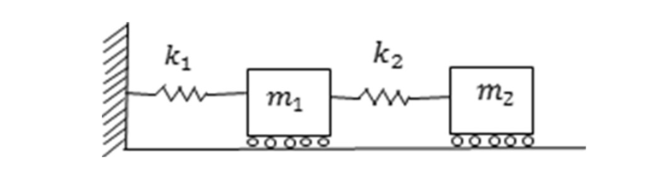
\includegraphics[width=\columnwidth]{figs/g54.fig1.png}
    \caption{ }
    \label{}
\end{figure}                   
\\    \hfill{GATE NM 2022} \\

\solution

\begin{figure}[!ht]
    \centering
    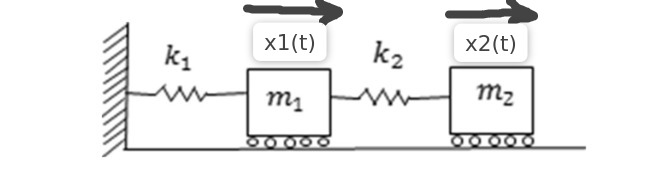
\includegraphics[width=\columnwidth]{figs/g54.fig2.jpeg}
    \caption{ }
    \label{}
\end{figure} 

\begin{table}[!ht]    
    \centering
    \resizebox{9cm}{2cm}{
            \begin{tabular}{|c|c|c|} 
    \hline
\textbf{Variable} & \textbf{Description} & \textbf{Value} \\\hline
    $m_1$ & Mass of block 1 & $200kg$  \\\hline
    $m_2$ & Mass of block 2 & $100kg$  \\\hline
    $k_1$ & Stiffness coefficient of spring$1$ & $200N/m$  \\\hline
    $k_2$ & Stiffness coefficient of spring$2$ & $200N/m$  \\\hline
    $x_i(t)$ & Displacement of $i^{th}$ block & $x_i(t)=\cos \brak{\omega t +\phi _i}$,$x_i\geq 0$ \\ \hline
        \end{tabular}
    
    
 
    }
    \caption{Input Parameters}
    \label{table:ishitha.g22.nm.54.t1}
\end{table}


\begin{align}
m_2\ddot{x_2}(t) + k_2\brak{x_2(t)-x_1(t)}&=0
\label{eq:ishitha.g22.nm.54.1.eq} \\
m_1\ddot{x_1}(t) - k_2\brak{x_2(t)-x_1(t)}+ k_1x_1(t)&=0
\label{eq:ishitha.g22.nm.54.2.eq}
\end{align}

Writing ~\eqref{eq:ishitha.g22.nm.54.1.eq} and ~\eqref{eq:ishitha.g22.nm.54.2.eq} in matrix form:
\[
\begin{bmatrix}
m_1 & 0  \\
0 & m_2
\end{bmatrix}
\begin{bmatrix}
\ddot{x_1}(t) \\
\ddot{x_2}(t)
\end{bmatrix}
+
\begin{bmatrix}
k_1+k_2 & -k_2  \\
-k_2 & k_2
\end{bmatrix}
\begin{bmatrix}
x_1(t) \\
x_2(t)
\end{bmatrix}
=
\begin{bmatrix}
0 \\
0
\end{bmatrix}
\]
From above ;
\begin{align}
x_1(0)&=0 
 \label{eq:ishitha.g22.nm.54.3.eq} \\
x_2(0)&=0 
\label{eq:ishitha.g22.nm.54.4.eq} \\
\ddot{x_1}(0)&=0 
\label{eq:ishitha.g22.nm.54.5.eq} \\
\ddot{x_2}(0)&=0
\label{eq:ishitha.g22.nm.54.6.eq} 
\end{align}

\begin{equation}
x(t)     \systemL{}   X(s)  
\end{equation}


\begin{equation}
x^{''}(t) \systemL{} s^{2}X(s)-sx(0)-x^{'}(0)
\end{equation}

From ~\eqref{eq:ishitha.g22.nm.54.3.eq} and ~\eqref{eq:ishitha.g22.nm.54.5.eq}
\begin{align}
X_1(0)&=0\\
s^{2}X_1(0)-sx_1(0)-x_1^{'}(0)&=0\\
\implies x_1^{'}(0)&=0
\end{align}

From ~\eqref{eq:ishitha.g22.nm.54.4.eq} and ~\eqref{eq:ishitha.g22.nm.54.6.eq}
\begin{align}
X_2(0)&=0\\
s^{2}X_2(0)-sx_2(0)-x_2^{'}(0)&=0\\
\implies x_2^{'}(0)&=0
\end{align}

Applying Laplace transform for ~\eqref{eq:ishitha.g22.nm.54.1.eq} and ~\eqref{eq:ishitha.g22.nm.54.2.eq}
\begin{align}
m_1s^2X_1(s) - k_2\brak{X_2(s)-X_1(s)} + k_1X_1(s) &= 0
\label{eq:ishitha.g22.nm.54.7.eq} \\
m_2s^2X_2(s) + k_2\brak{X_2(s)-X_1(s)}&=0
\label{eq:ishitha.g22.nm.54.8.eq} 
\end{align}

Writing ~\eqref{eq:ishitha.g22.nm.54.7.eq} and ~\eqref{eq:ishitha.g22.nm.54.8.eq} in matrix form:
\[
\begin{bmatrix}
m_1s^2+(k_1+k_2) & -k_2  \\
-k_2& m_2s^2+k_2
\end{bmatrix}
\begin{bmatrix}
X_1(s) \\
X_2(s)
\end{bmatrix}
=
\begin{bmatrix}
0 \\
0
\end{bmatrix}
\]

For frequency put $s=j\omega$,
\[
\begin{bmatrix}
-m_1\omega ^2+(k_1+k_2) & -k_2  \\
-k_2& -m_2\omega ^2+k_2
\end{bmatrix}
\begin{bmatrix}
X_1(j\omega) \\
X_2(j\omega)
\end{bmatrix}
=
\begin{bmatrix}
0 \\
0
\end{bmatrix}
\]

For free vibration 
\[
\det
\begin{pmatrix}
-m_1\omega^2+(k_1+k_2) & -k_2 \\
-k_2 & -m_2\omega^2+k_2
\end{pmatrix}
= 0
\]

\begin{align}
\brak{-m_1\omega^2+(k_1+k_2)}\brak{-m_2\omega^2+k_2}-\brak{-k_2}\brak{-k_2}&=0 \\
m_1m_2\omega ^4 -\sbrak{\brak{k_1+k_2}m_2+k_2m_1}\omega^2 +k_1k_2&=0\\
\implies \omega ^4 -\frac{\sbrak{\brak{k_1+k_2}m_2+k_2m_1}}{m_1m_2}\omega^2 +\frac{k_1k_2}{m_1m_2}&=0
\end{align}

Substituting the values;
\begin{align}
\implies \omega ^4 -4\omega^2 +2&=0 \\
\omega ^2 &= \frac{4\pm \sqrt{16-8}}{2}\\
&= 2\pm \sqrt{2}\\
 \omega &= \pm \sqrt{2\pm \sqrt{2}}\\
\implies \omega_{least} &= 0.765 rad/s
\end{align}
\end{document}
